\documentclass{article}

\usepackage{graphicx}
\usepackage{subcaption}
\usepackage{amsmath}
\usepackage{amsfonts}

\begin{document}

\author{Zachary Vogel}
\date{\today}
\title{Notes in APPM 4650\\Adam Norris}

\maketitle



\section{Moar on project}
conservation in the project:
mass $u_x+v_y=0$, $\delta_v=0$\\
x-momentum $uu_x+vu_y=\nu u_{yy}$\\
Fe energy $uT_x+vT_y=\alpha T_{yy}$\\
$y\to\infty$ far field.\\
Similarity Transform to:\\
\[\eta=\cfrac{y}{\sqrt{\frac{\nu x}{u_\infty}}}\]
\[\frac{u}{u_\infty}=F'(\eta)\]
\[v=\frac{1}{2}\sqrt{\frac{vu_\infty}{x}}(\eta F'(\eta)-F(\eta))\]
\[G=\frac{T-T_\infty}{T_{wall}-T_\infty}\]
\[F'''+\frac{1}{2}FF''=0\]
\[G''+\frac{Pr}{2}FG'=0\]

boundary conditions from last time.\\
note that F can be solved without G.\\
garden hose or shooting technique to get better initial conditions\\
guess on the slope of $F''$, solve the problem, see if it matches the value of $F'$ at infinity. Guess again, repeat till it's correct.\\
wants six figures of accuracy on this. So with your guess, it should give you 1.000000 at the very least.\\

do the same thing once you have the solution of $F$.\\
G has to asymptote to $0.000000$.\\

Want to find $\eta_m$ such that $F'$ is $0.9700000$. Somewhere in G there is a $\eta_T$ that gives you $G=0.0300000$.\\
\begin{figure}[h!]
    \centering
    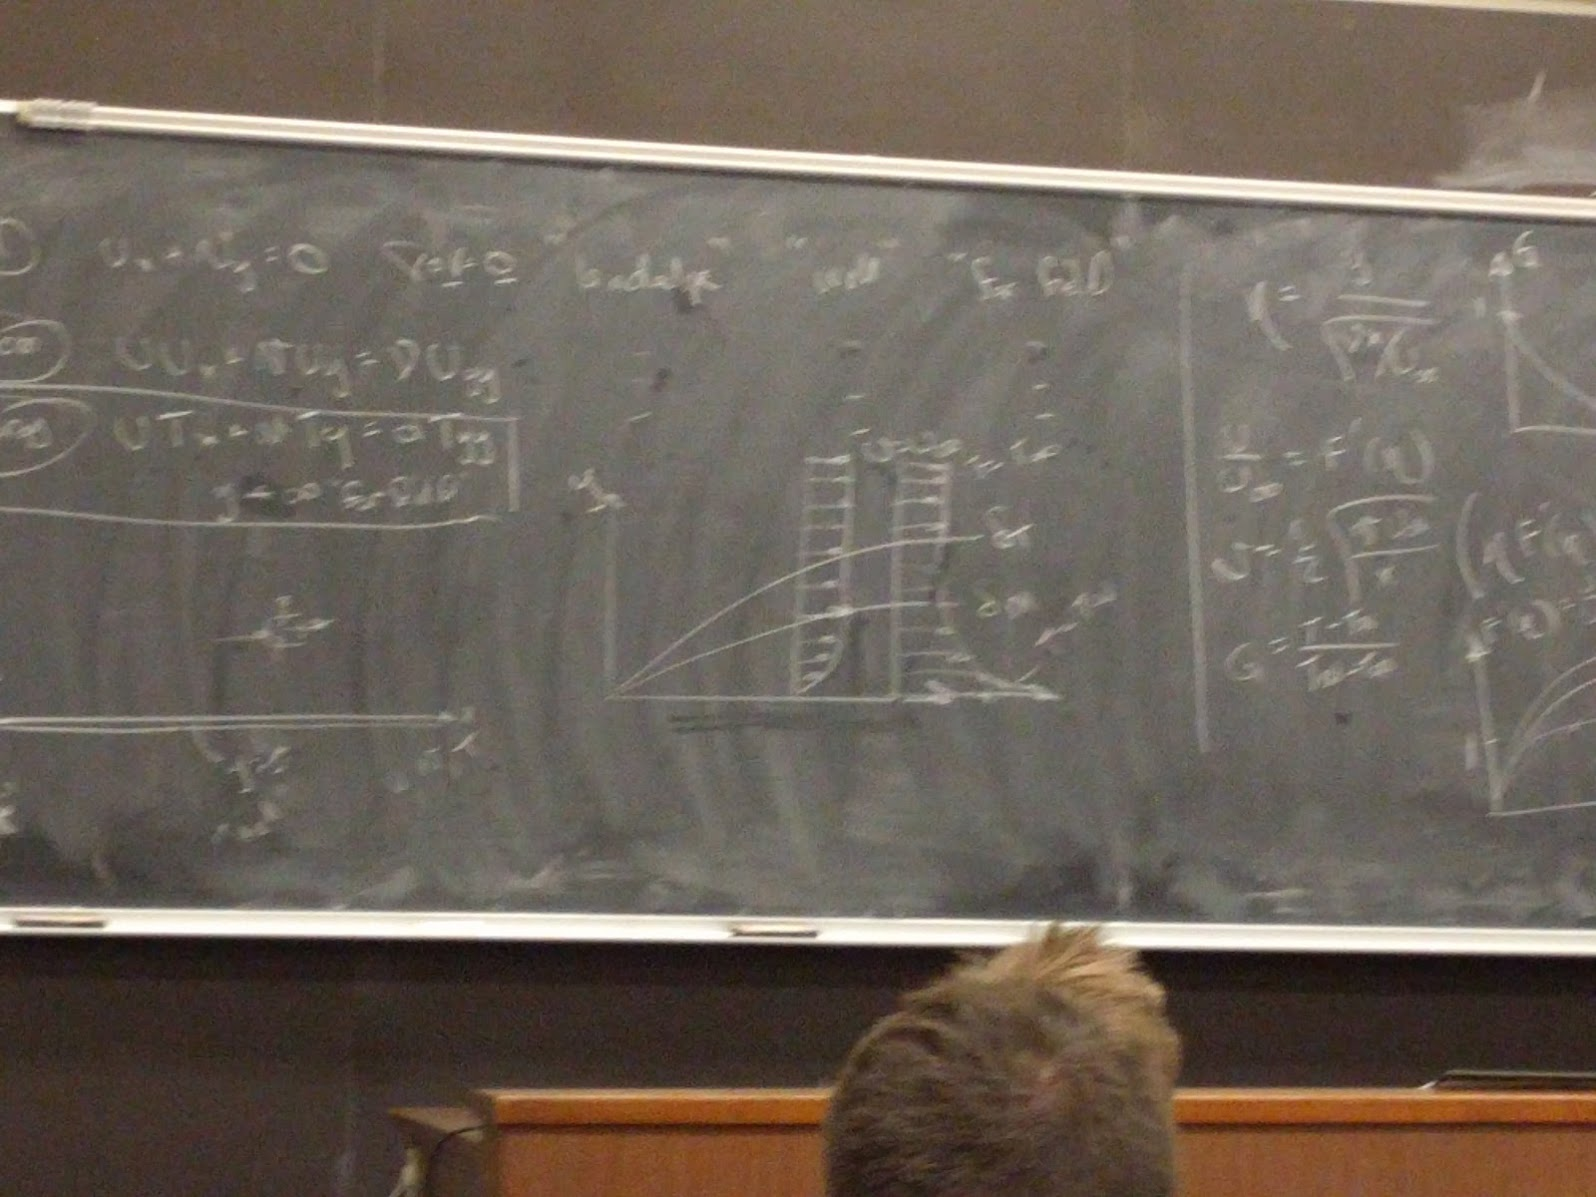
\includegraphics[width=0.8\textwidth,clip=true,trim={17cm 15cm 15cm 14cm}]{proj21.jpg}
\end{figure}
\begin{figure}[h!]
    \centering
    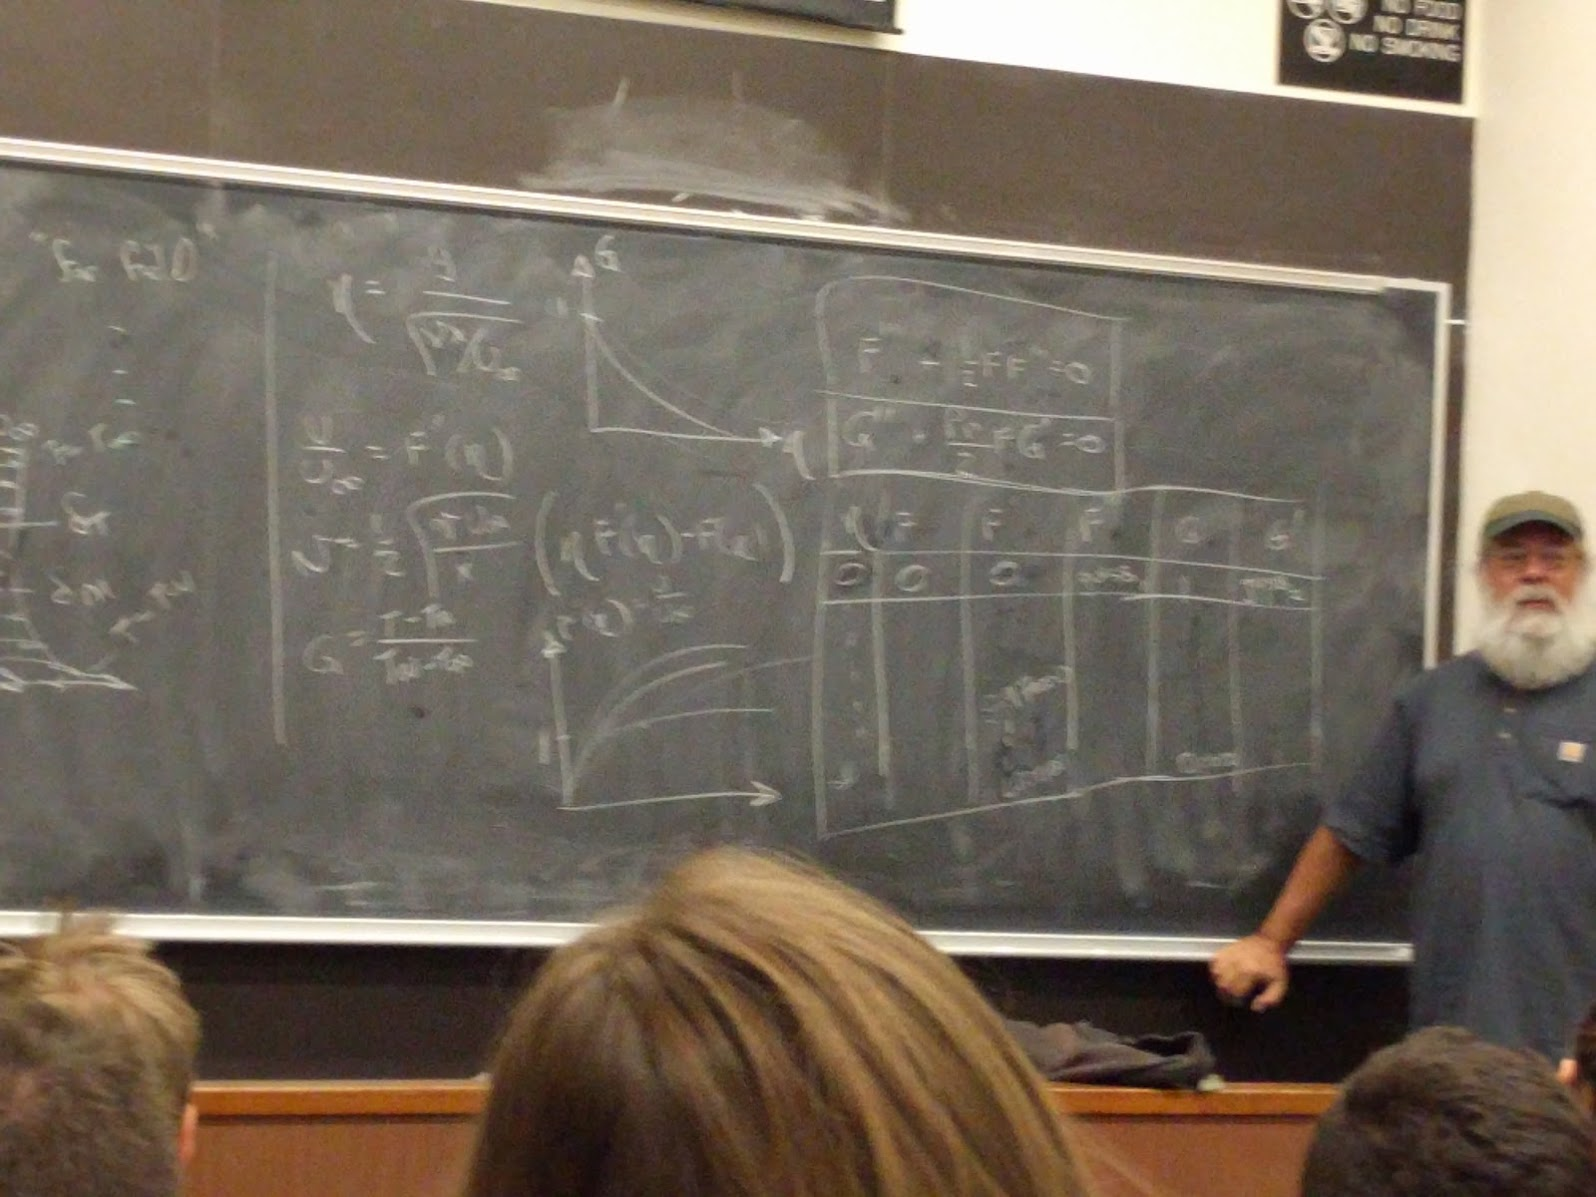
\includegraphics[width=0.8\textwidth,clip=true,trim={22cm 9cm 7cm 15cm}]{proj22.jpg}
\end{figure}

There is a problem because the Prandtl number changes $Pr=\frac{\nu}{\alpha}$.\\
The $\eta_m$ stays the same, but $\eta_T$ changes. He wants a table of these values for the various Prandtl numbers.\\
Once you get the graph of $F'$ vs $\eta$ that asymptotes to 1. He wants a graph of $\eta F'(\eta)-F(\eta)$.\\
If the PR number is 1 than we have two of the same differential equations only with different initial conditions.\\
At this point $\eta_T=\eta_m$.\\


\end{document}
